\chaptercover{Related Work}{chap:RelatedWork}
{In this chapter, we explore the concepts and state of the art concerning the topics that relate to our intended work, which allow us to have a better understanding of the problem under study. This chapter is organized in 5 sections, structured as follows. Section~\ref{sec:RelatedWork-ModelDrivenDevelopment} starts by presenting the main concepts of Model-Driven Development, including the definition of UML, and OCL. Section~\ref{sec:RelatedWork-UML} covers existing studies on comprehension of UML Class Diagrams, and the impact of OCL on UML-based development. Section~\ref{sec:RelatedWork-Metrics} discusses the complexity of OCL expressions and presents existing metrics proposed by experts to calculate this complexity. Section~\ref{sec:RelatedWork-SyntaxHighlight} examines relevant papers on the impact of syntax highlighting on program comprehension. Finally, Section~\ref{sec:RelatedWork-OCLTools} presents some OCL support tools and their functionalities.}
%%%%%%%%%%%%%%%%%%%%%%%%%%%%%%%%%%%%%%%%%%%%%%%%%%%%%%%%%%%%%%%%%%%%%%%%%%%%%%

%\chapterquotes{...All things -from the tiniest virus to the greatest galaxy- are, in reality, not things at all, but processes...}{In \textit{"Future Shock"}, 1970.}{Alvin Toffler(1928-2016)}{American writer, futurist, and businessman known for his works discussing modern technologies, including the digital and the communication revolutions, with emphasis on their effects on cultures worldwide.}

To identify all relevant studies for our topic, we started by defining the search strategy, which states that the title, abstract, and keywords of the articles, books, and conference proceedings will be searched in the appropriate electronic databases (IEEE Xplore, ACM Digital Library, Elsevier, Springer, ...) according to the following search~\textit{string}: 

((("uml" AND "class diagram") OR "ocl" OR "program") AND ("comprehension" OR "complexity" OR "highlight")) OR ("ocl" AND "tool")
%((("uml" AND "class diagram") OR "ocl" OR "program") AND ("comprehension" OR "complexity" OR ("eye" AND "tracking") OR "highlight")) OR ("ocl" AND "tool")

To only select articles that are pertinent to our topic, the following inclusion/exclusion criteria were applied: if the abstract of the article is not clearly related with the topic under study, or if it wasn't published by a top publisher (e.g. IEEE, ACM, Wiley, Springer, Elsevier), then the article wasn't considered. Additionally, we used forward snowballing whenever the references of the selected articles were relevant in the context of this dissertation.

\section{Concepts of Model-Driven Development} 
\label{sec:RelatedWork-ModelDrivenDevelopment}

Model-Driven Development is presented as the methodology of software development with models as the primary focus, rather than computer programs. Models are artefacts used to specify the system's required functionality and architecture and to guide the development of the final piece of software. Since these models are closer to the problem domain, abstracted from the underlying technologies, they are a high-level specification, easier to specify, understand and maintain~\cite{mda2014}~\cite{Selic2003}~\cite{Atkinson2003}.

To express the necessary information of a system, models need to be represented in a way that can be comprehended by modellers, developers, stakeholders, and other supporting systems. A modelling language is either a graphical or textual computer language that allows the creation of models, following a specific set of structures, terms, notations, syntaxes, semantics, and integrity rules~\cite{mda2014}. There are many well-known modelling languages, including~\gls{bpmn}, SQL Schema,~\gls{xml} Schema, and UML~\cite{uml2005}. UML is currently accepted as the standard graphical notation for software development, but its diagrams cannot express all constraints and essential aspects of a system precisely. To address the existing flaws in UML diagrams, IBM proposed Object Constraint Language~\cite{ocl2014}, which is now part of the UML standard. OCL is a "semi-formal" language since it lacks inference mechanisms (second-order logic), that allows specification of invariants, pre-and post-conditions as well as the description of guards and constraints on operations.

\section{UML Class Diagrams comprehension} 
\label{sec:RelatedWork-UML}

Over the years, several studies have been conducted to assess how software engineers build, understand, and design programs. In the topic of program comprehension, we're particularly interested in addressing how humans process class diagrams to acquire information about a system. Class Diagrams, which are one type of UML diagrams, describe the structure and global behaviour of a program by showing it's classes, attributes, operations, and relationships, hence this type of diagram is useful for both modelling and understanding of a program.  
Guehénéuc~\cite{Gueheneuc2006} and Yusuf~\cite{Yusuf2007} used eye-tracking technology to obtain data on how subjects process UML Class Diagrams, namely how they explore, visualize and examine data. Sight is the most important sense in this process, which makes it relevant to study the behaviour of the human eye. Three types of information are particularly relevant: fixations, saccades, and scanpaths. Fixations are defined by a period of time where the subject maintains the visual gaze on a single location, represented by a pair of coordinates; saccades involve a quick movement between two fixation points; finally, scanpaths are defined as directed paths formed by saccades between fixations. Results of eye-tracking studies can be represented as shown: Figure \ref{fig:01_gazeplot} shows a gaze plot of a UML class diagrams with fixations, saccades, and scanpaths, whereas Figure~\ref{fig:02_heatmap} shows a heatmap of fixations. By analyzing these two figures, it's possible to discern the path taken by the subject's eyes through the diagram and which were the main focus points. This information is important when trying to understand how subjects visually process class diagrams. Relevant conclusions show that relationships mainly contain fixations on its ends and saccades on the line, indicating that lines are mainly used for navigation purposes. A large number of fixations on a \textit{stimulus}, an object that is viewed by a subject, indicate a greater effort to understand the object in question, due to either its complexity or the poor layout arrangement. The use of colour information was found useful for experts when trying to explore class diagrams more efficiently.

%\plot{chapter6/chapter6-1.pdf}[ProcessLabs Portfolio covers Software Development Process Mining][9][H][trim=0cm 0cm 0cm 0cm]

\begin{figure}[ht]
\centering
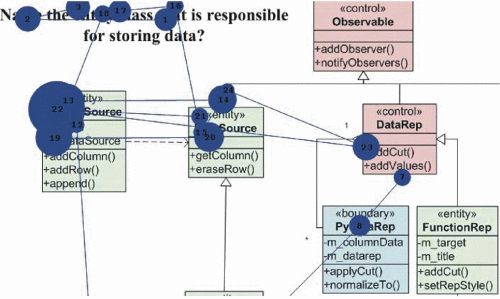
\includegraphics[width=0.7\textwidth]{Template/Chapters/figures/4_RelatedWork/01_GazePlot.png}
\caption{Gaze plot of a UML class diagram exploration~\cite{Yusuf2007}}
\label{fig:01_gazeplot}
\end{figure}

\begin{figure}[ht]
\centering
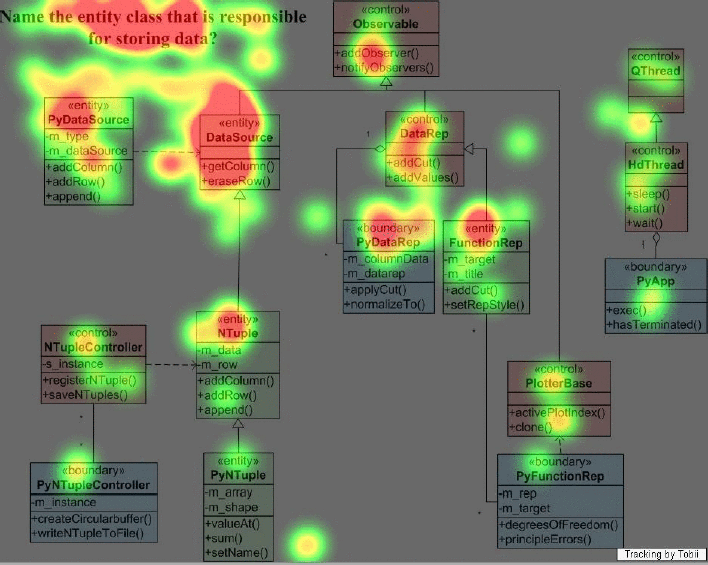
\includegraphics[width=0.7\textwidth]{Template/Chapters/figures/4_RelatedWork/02_HeatMap.png}
\caption{Heatmap of a UML class diagram exploration~\cite{Yusuf2007}}
\label{fig:02_heatmap}
\end{figure}

Comprehension of UML Class Diagrams is particularly important when designing and maintaining OCL expressions because they're always tied to the context of this type of diagram. These expressions can be used to specify objects' invariants and pre-and post-conditions on operations, and also to query the system data to return information to the user. The impact of OCL in UML-based development has been discussed throughout many investigations over the past years, focusing on OCL's influence on comprehension and maintainability of UML models, and whereas the additional effort and formality justify the benefit. Briand et al. ~\cite{Briand2004,Briand2005} investigated the impact of OCL during development, understanding, and modification of UML analysis documents, which are three typical software engineering activities. The authors compared subjects (\nth{4} year software/computer engineering students) performance on comprehension and maintenance tasks when using OCL to document invariants, pre-and post-conditions, which are typically documented in NL. Results showed that OCL has the potential to promote comprehension and modification of UML diagrams, but requires a high level of experience and training.

\section{Metrics for OCL expressions} 
\label{sec:RelatedWork-Metrics}

The cognitive effort needed to comprehend, design, and/or maintain systems is influenced by the levels of complexity that characterize OCL expressions. There has been an ongoing effort to define OCL complexity metrics~\cite{Reynoso2005Book}, and to study how they can capture different levels of comprehensibility and maintainability of OCL expressions. Reynoso et al. ~\cite{Reynoso2005, Reynoso2010} pursued insight in the process of understanding OCL expressions by applying the techniques of chunking (which involves recognizing groups of declarations and the extraction of information, that is remembered as a chunk) and tracing (which involves scanning through a program in different directions in search of relevant chunks). While there are many distinct metrics that capture different aspects that affect expression's complexity, these authors decided to focus on the impact of tracing-based metrics, because this technique was proven as an essential activity in program comprehension~\cite{Reynoso2005Book}. They found statistical significance on the impact of tracing-related metrics on the understandability and, consequently, modifiability of OCL expressions. The process is shown in Figure~\ref{fig:03_oclcomplexity}: the structural properties of an OCL expression affect the cognitive complexity needed to comprehend that expression, which consequently influences understandability and maintainability. Table~\ref{tbl:tracingMetrics} shows the metrics in question and their classifications, depending on their focus on the structural properties of OCL expressions: coupling (degree of interdependence between objects), size, and length.

\begin{figure}[ht]
\centering
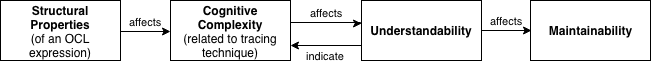
\includegraphics[width=0.9\textwidth]{Chapters/figures/4_RelatedWork/03_OCLComplexity.png}
\caption{Relationship between structural properties of an OCL expression, cognitive complexity related to tracing, understandability and maintainability (based on~\cite{Reynoso2005Book})}
\label{fig:03_oclcomplexity}
\end{figure}

%\begin{table}[ht]
\centering
\begin{threeparttable}  
\caption{Tracing-related OCL expression metrics (based on~\cite{Reynoso2005Book})}
\label{tbl:tracingMetrics}
\begin{tabular}{@{}lll@{}}
\toprule
\begin{tabular}[c]{@{}l@{}}Metric \\ Acronym\end{tabular} & \begin{tabular}[c]{@{}l@{}}Metric \\ Description\end{tabular}                                                      & \begin{tabular}[c]{@{}l@{}}Metric \\ Classification\end{tabular} \\ \midrule
NNR                                                       & Number of Navigated Relationships                                                                                  & C                                                                \\
NAN                                                       & Number of Attributes referred through Navigations                                                                  & C                                                                \\
WNO                                                      & \begin{tabular}[c]{@{}l@{}}Weighted Number of referred Operations \\ through Navigations\end{tabular}              & C                                                                \\
NNC                                                       & Number of Navigated Classes                                                                                        & C                                                                \\
WNM                                                       & Weighted Number of Messages                                                                                        & C, S                                                             \\
NPT                                                       & \begin{tabular}[c]{@{}l@{}}Number of Parameters whose Types are classes\\  defined in a class diagram\end{tabular} & C                                                                \\
NUCA                                                      & Number of Utility Classes Attributes Used                                                                          & C                                                                \\
NUCO                                                      & Number of Utility Classes Operations Used                                                                          & C                                                                \\
DN                                                        & Depth of Navigations                                                                                               & L                                                                \\
WNN                                                       & Weighted Number of Navigations                                                                                     & S                                                                \\
WCO                                                       & Weighted Number of Collection Operations                                                                           & S                                                                \\ \bottomrule
\end{tabular}
\begin{tablenotes}
    \small
    \item Note: In the table above, C stands for Coupling, S stands for Size, and L stands for Length.
\end{tablenotes}
\end{threeparttable} 
\end{table}

\begin{table}[ht]
\centering
\begin{threeparttable}  
\caption{Tracing-related OCL expression metrics (based on~\cite{Reynoso2005Book})}
\label{tbl:tracingMetrics}
\begin{tabular}{@{}lll@{}}
\toprule
\begin{tabular}[c]{@{}l@{}}Metric \\ Acronym\end{tabular} & \begin{tabular}[c]{@{}l@{}}Metric \\ Description\end{tabular}                                                      & \begin{tabular}[c]{@{}l@{}}Metric \\ Classification\end{tabular} \\ \midrule
NNR                                                       & Number of Navigated Relationships                                                                                  & C                                                                \\
NAN                                                       & Number of Attributes referred through Navigations                                                                  & C                                                                \\
WNO                                                      & \begin{tabular}[c]{@{}l@{}}Weighted Number of referred Operations \\ through Navigations\end{tabular}              & C                                                                \\
NNC                                                       & Number of Navigated Classes                                                                                        & C                                                                \\
WNM                                                       & Weighted Number of Messages                                                                                        & C, S                                                             \\
NPT                                                       & \begin{tabular}[c]{@{}l@{}}Number of Parameters whose Types are classes\\  defined in a class diagram\end{tabular} & C                                                                \\
NUCA                                                      & Number of Utility Classes Attributes Used                                                                          & C                                                                \\
NUCO                                                      & Number of Utility Classes Operations Used                                                                          & C                                                                \\
DN                                                        & Depth of Navigations                                                                                               & L                                                                \\
WNN                                                       & Weighted Number of Navigations                                                                                     & S                                                                \\
WCO                                                       & Weighted Number of Collection Operations                                                                           & S                                                                \\ \bottomrule
\end{tabular}
\begin{tablenotes}
    \small
    \item Note: In the table above, C stands for Coupling, S stands for Size, and L stands for Length.
\end{tablenotes}
\end{threeparttable} 
\end{table}


The definition of these metrics is described below, based on~\cite{Reynoso2005Book}:

\begin{definition}\label{def:NNR}
NNR Metric (Number of Navigated Relationships): Measures the total number of navigated relationships in an expression. Relationships are only counted once, even if they're navigated multiple times.
\end{definition}

\begin{definition}\label{def:NAN}
NAN Metric (Number of Attributes referred through Navigations): Counts the number of attributes referred through navigations.
\end{definition}

\begin{definition}\label{def:WNO}
WNO Metric (Weighted Number of referred Operations through navigations): Measures the sum of weighted operations (where the weight is defined by the number of \textit{in/out} parameters,  including the return type) mentioned through navigations.
\end{definition}

\begin{definition}\label{def:NNC}
NNC Metric (Number of Navigated Classes): Measures the number of classes, association classes or interfaces referred through navigations.
\end{definition}

\begin{definition}\label{def:WNM}
WNM Metric (Weighted Number of Messages): This metric is defined as the sum of weighted messages (where the weight is defined by the number of parameters) present in an expression.
\end{definition}

\begin{definition}\label{def:NPT}
NPT Metric (Number of Parameters whose Types are classes defined in the class diagram): This metric is particularly used in pre- and post-conditions, and it counts the number of different classes and interfaces used as \textit{in/out} parameters or result.
\end{definition}

\begin{definition}\label{def:NUCA}
NUCA Metric (Number of Utility Class Attributes used): Measures the number of utility classes' attributes used in an expression. Attributes that belong to the same utility class are only counted once, even if they're referred multiple times.
\end{definition}

\begin{definition}\label{def:NUCO}
NUCO Metric (Number of Utility Class Operations used): This metric definition is similar to the NUCA metric, but instead of attributes it considers operations.
\end{definition}

\begin{definition}\label{def:DN}
DN Metric (Depth of Navigations): Measures the maximum depth of a navigation tree, where the root node represents the class name of the contextual instance (\textit{self}). For each navigation that starts from \textit{self}, we create a branch that connects to a new node, which represents the navigated class. A new tree is created if a navigation contains a collection operation defined in terms of new navigation(s), and it's connected to the original tree through a “definition connection”.
\end{definition}

\begin{definition}\label{def:WNN}
WNN Metric (Weighted Number of Navigations):  This metrics is defined as the sum of weighted navigations presented in an expression, where the weight is defined by the level on which the operation is used in an expression.
\end{definition}

\begin{definition}\label{def:WCO}
WCO Metric (Weighted Number of Collection Operations): Measures the sum of weighted collection operations, where the weight is defined by the level on which the operation is used in an expression.
\end{definition}

Later in this document (subsection~\ref{Results-OCLComplexityMetrics}), we present the results of our investigation on the influence of these metrics on the success/failure of bachelor students when answering OCL questionnaires. We decided to include as a contribution of this dissertation a plugin for Bremen's USE tool~\cite{use} that allows modellers to evaluate OCL expressions and get the calculated complexities given by these metrics. The implementation details are described in section~\ref{chap:Implementation-OCLComplexityPlugin}.

\section{Impact of syntax highlighting on program comprehension}
\label{sec:RelatedWork-SyntaxHighlight}

In the context of this dissertation, it is not only important to understand what affects the comprehensibility of UML Class Diagrams and OCL expressions, but also to investigate the effort that has been made to improve program comprehension. The tasks of understanding and maintaining software systems are greatly influenced by the levels of readability and comprehensibility of programs. These can be affected by many factors, including naming scheme, indentation, commenting, and documentation. This section focuses on relevant research findings on the impact of syntax highlighting in program readability and comprehension. Syntax highlighting is a feature present in several text editors that allow displaying text in different colours (including background colour) and fonts depending on its categorization, making it easily distinguishable from other types of text without affecting the behaviour of the code. Figure~\ref{fig:06_syntaxhighligh1} shows the same code snippet with and without syntax highlight. On the right side the important keywords, e.g. \textit{while} or \textit{print}, and the comment are easily detected, comparing to the rest of the code, because they are displayed in different colours.

\begin{figure}[ht]
\centering
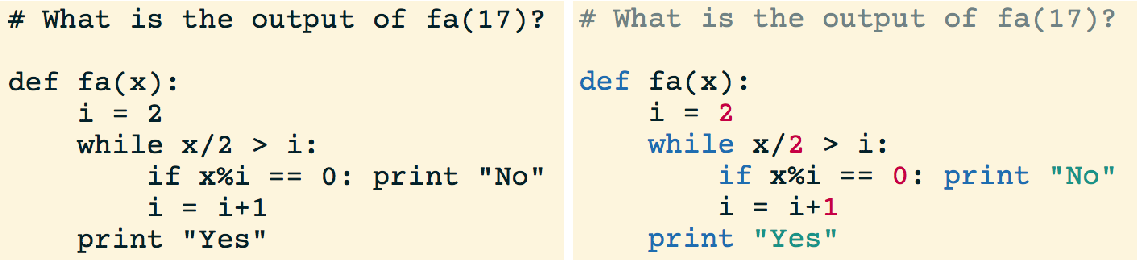
\includegraphics[width=0.9\textwidth]{Chapters/figures/4_RelatedWork/04_SyntaxHighlight1.png}
\caption{Same code with (right) and without (left) syntax highlighting~\cite{Sarkar2015}}
\label{fig:06_syntaxhighligh1}
\end{figure}

Initial studies were mainly concerned with the effect of colours on program comprehension in order to facilitate the learning process and increase developers' productivity, as the majority of tools was only available in black and white. Rambally~\cite{Rambally1986} studied the effect of two colour schemes on program comprehension when compared to a version of the same program presented in black and white: Color-scheme-A used different colours for code blocks, e.g. loops and conditionals; Color-scheme-B used different colours to identify statements and functions, e.g. I/O (Input/Output), decision and declaration statements, and variable binding. From a sample of 44 intermediate-level (novice) and 35 senior-level (expert) programming students, results showed that, in general, both groups could better understand programs when using Color-scheme-B. An interesting note mentioned in this experiment is that the participants subjectively favoured Color-scheme-A as the easiest to understand, even tough results supported Color-scheme-B as the most effective for the completion of the given comprehension tasks.

Several years after this research, Sarkar~\cite{Sarkar2015} did an experiment to evaluate the impact of syntax colouring on program comprehension time, using ten graduate computer science students. Even though the experiment's validity is threatened by the small number of participants, it showed that assignments were solved remarkably faster when using syntax highlighting. The author collected the participants' sessions with an eye-tracking device and discerned that syntax highlighting directed participants' focus on to smaller regions of the code (see Figure~\ref{fig:06_syntaxhighligh2}). In some cases, even some keywords were completely ignored, as seen in Figure~\ref{fig:06_syntaxhighligh3}. Another interesting remark taken from this investigation is that the benefits of syntax highlighting in novice programmers are significantly more relevant when compared to experienced programmers, which might indicate that it's a useful feature when learning a certain language, but less important for using it.

\begin{figure}[ht]
\centering
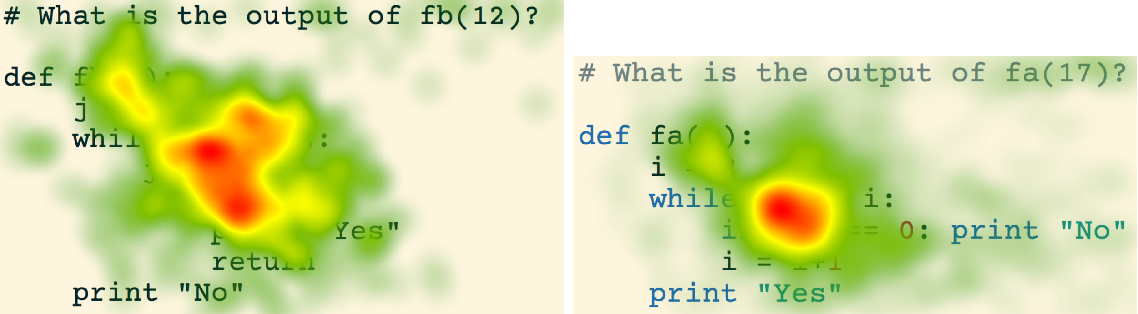
\includegraphics[width=0.9\textwidth]{Chapters/figures/4_RelatedWork/04_SyntaxHighlight2.png}
\caption{Fixation heat map for the same code without (left) and with (right) syntax highlighting~\cite{Sarkar2015}}
\label{fig:06_syntaxhighligh2}
\end{figure}

\begin{figure}[ht]
\centering
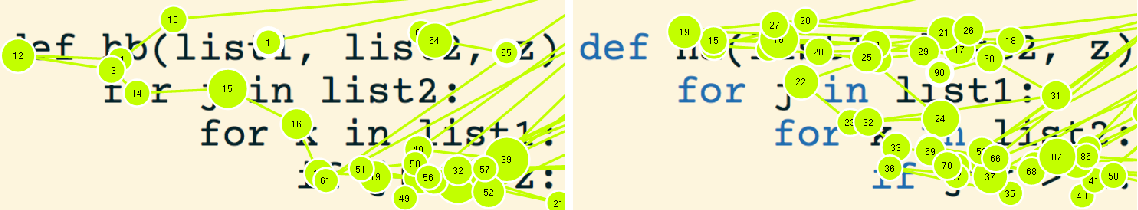
\includegraphics[width=0.9\textwidth]{Chapters/figures/4_RelatedWork/04_SyntaxHighlight3.png}
\caption{Gaze plot for the same code without (left) and with (right) syntax highlighting. The numbers represent the order in which the fixations occurred~\cite{Sarkar2015}}
\label{fig:06_syntaxhighligh3}
\end{figure}

An important aspect when using syntax highlighting is to decide which features to include and how to code them. It's essential to determine which is the most efficient way to display certain information, e.g. choosing to use colour X over Y for a specific category of information, selecting a background colour instead of a text colour, ... Mehta and Zhu~\cite{Mehta2009} focus on the effect of colours (red and blue) on cognitive task performance. They start by describing the theory defended by colour theorists which states that people create specific associations to colours depending on the repeated situations they experience with that colour: red is an intensive colour normally associated with errors or dangers, while blue is mostly associated with calmness, peace, and tranquillity. Results from this research show that distinct colours offer different benefits, and the choice of the right colour depends on the nature of the task. As red primarily activates an avoidance motivation, it mainly enhances performance on detail-oriented tasks. On the other hand, blue activates an approach motivation which is more beneficial for creative tasks.

In summary, previous research shows that visual coding hints through syntax highlighting can improve program comprehension, and consequently reduce the time needed to complete a given task, especially for novice developers. Many distinct features can be used (e.g. colour, font size, ...), but it's important to understand the different effects they provoke on people so that we can choose the appropriate feature depending on the desired outcome. As one of the main goals of this dissertation is to soften OCL's learning curve, we developed a second plugin for USE, this time providing syntax highlight to the elements of a UML Class Diagram referenced by an OCL expression. The implementation details are presented in section~\ref{chap:Implementation-OCLHighlightPlugin}, and the experiments of it's success described in subsection~\ref{chap:Results-OCLHighlightPlugin}.

\section{OCL tools}
\label{sec:RelatedWork-OCLTools}

Currently, there are several OCL tools available, either freely or for commercial use, that assist modellers in the development, analysis, and maintenance of systems. It's important to investigate their main functionalities to understand what this dissertation can offer to the current body of knowledge. Toval et al. ~\cite{Toval2003} defined a set of features found desirable when working with OCL and presented a comparison of the main characteristics (shown in Table~\ref{tbl:oclToolsCharacteristics}) of the existing tools. In the meantime, some of them received updates (for example, to support newer versions of OCL), some had their development cancelled or were integrated into other systems, and other tools emerged. For our topic, we're mainly interested in the available features of the two most common OCL tools, which are USE (UML-based Specification Environment)~\cite{use}, and Eclipse OCL~\cite{eclipseocl}.

\begin{table}[ht]
\centering
\begin{threeparttable}  
\caption{Main OCL tools characteristics (based on~\cite{Toval2003})}
\label{tbl:oclToolsCharacteristics}
\begin{tabular}{@{}lccc@{}}
\toprule
\multicolumn{1}{c}{Analysis}                                 & Communication                                                       & Features                                                                              & \begin{tabular}[c]{@{}c@{}}Dynamic \\ validation\end{tabular}                     \\ \midrule
\begin{tabular}[c]{@{}l@{}}Syntatic \\ analysis\end{tabular} & Model-independent                                                   & \begin{tabular}[c]{@{}c@{}}Guided support \\ for constraint \\ development\end{tabular} & \begin{tabular}[c]{@{}c@{}}Invariant \\ validation\end{tabular}                   \\
\begin{tabular}[c]{@{}l@{}}Type \\ checking\end{tabular}     & \begin{tabular}[c]{@{}c@{}}With connection \\ to model\end{tabular} & \begin{tabular}[c]{@{}c@{}}Code generation \\ from OCL \\ specifications\end{tabular}   & \begin{tabular}[c]{@{}c@{}}Consistent \\ checking \\ of contraints\end{tabular}   \\
                                                             &                                                                     & \begin{tabular}[c]{@{}c@{}}Insertion of \\ OCL expressions*\end{tabular}                 & \begin{tabular}[c]{@{}c@{}}Pre- and \\ post-conditions \\ validation\end{tabular} \\ \bottomrule
\end{tabular}
\begin{tablenotes}
    \small
    \item * Includes three possibilities: imported from a UML model, imported from an independent file or manually introduced.
\end{tablenotes}
\end{threeparttable} 
\end{table}

USE is one of the pioneering OCL tools. It was initially developed in Java by Mark Richters as a dissertation project at the University of Bremen~\cite{Gogolla2007}. It's freely distributed under GPLv2 (GNU General Public License version 2.0), and the latest version, USE 6.0.0, was released in September 2020. Main functionalities include syntactic analysis, type checking, dynamic validation of invariants and pre-and post-conditions, and consistency checking. The core feature of USE is to validate specifications that consist of UML class diagrams and OCL expressions (invariants and pre-and post-conditions), which can be effective when helping modellers and developers in early development stages. It's also important to refer that USE allows the connection with UML models, which is made through a specific file (\textit{.use}). Additional functionalities include an evaluation browser (see Figure~\ref{fig:05_usetool2}), and syntax highlighting of the coverage of the expressions (see Figure~\ref{fig:05_usetool3}). The evaluation browser allows users to manually introduce OCL expressions and to debug them, as it generates an~\gls{ast} from the input text that is evaluated against the model and returns either a syntax error or the result of the given expression. These two features are the most important, in the context of this dissertation, because they provide the basis for the development of the plugin for syntax highlighting when evaluating OCL expressions in the evaluation browser. As a last remark, this tool allows third parties to contribute with additional functionalities through plugins.

\begin{figure}[ht]
  \centering
  \begin{tabular}{@{}c@{}}
    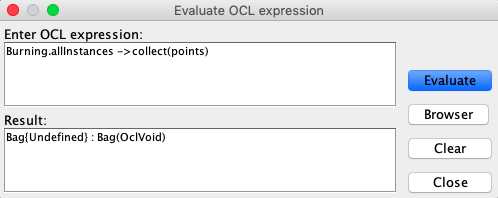
\includegraphics[width=.6\linewidth]{Chapters/figures/4_RelatedWork/05_USETool_1.png} \\[\abovecaptionskip]
    \small (a) Expression evaluation
  \end{tabular}

  \vspace{\floatsep}

  \begin{tabular}{@{}c@{}}
    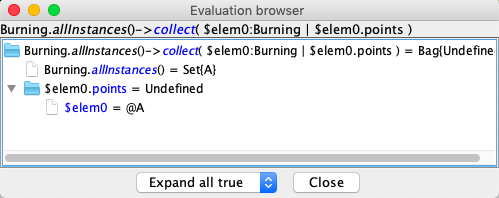
\includegraphics[width=.6\linewidth]{Chapters/figures/4_RelatedWork/05_USETool_2.png} \\[\abovecaptionskip]
    \small (b) Evaluation browser
  \end{tabular}

  \caption{Evaluation browser on USE (Royal and Loyal example from~\cite{Warmer2003})}\label{fig:05_usetool2}
\end{figure}

\begin{figure}[ht]
\centering
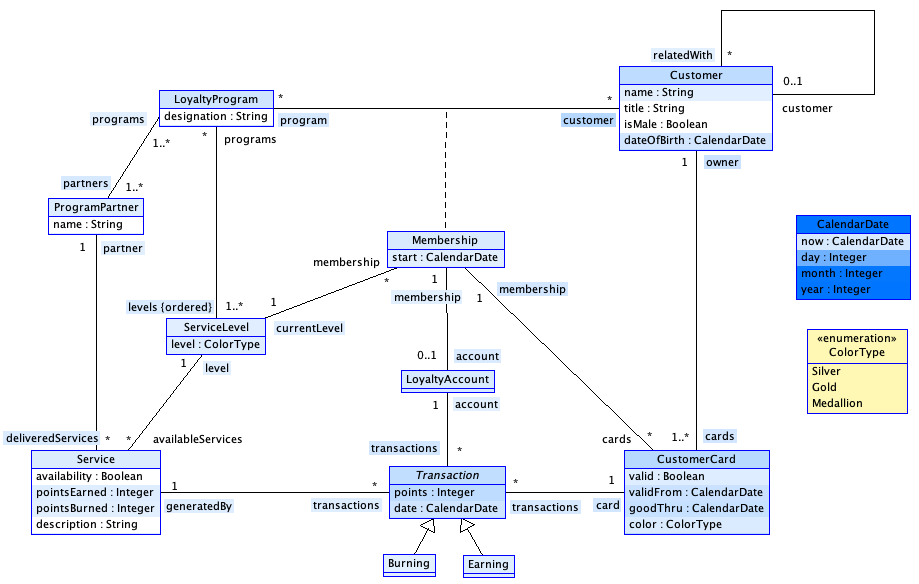
\includegraphics[width=0.9\textwidth]{Chapters/figures/4_RelatedWork/05_USETool_3.png}
\caption{View of class diagram with coverage (Royal and Loyal example from~\cite{Warmer2003})}
\label{fig:05_usetool3}
\end{figure}

As mentioned above, Eclipse OCL is also an important tool to analyze, as it's becoming the most popular OCL tool. It's part of the Eclipse Modeling Project, which focus on supporting model-driven development by presenting a consolidated set of modeling frameworks, tools, and standards implementations. It enables editing, refactoring, code generation, execution, and interactive debugging of OCL constraints, in the context of a class model. The dynamic input and evaluation of OCL expressions can not only be made on the OCL console (see Figure~\ref{fig:07_eclipseocl_1}) but also using the Java~\gls{api}. It also provides a debugger tool (see Figure~\ref{fig:07_eclipseocl_2}) that offers syntax highlighting with error indications, quick fixes, and content assist. Unfortunately, the available documentation doesn't refer syntax highlighting on the UML class diagram, which is the most important topic in the context of this dissertation.

\begin{figure}[ht]
\centering
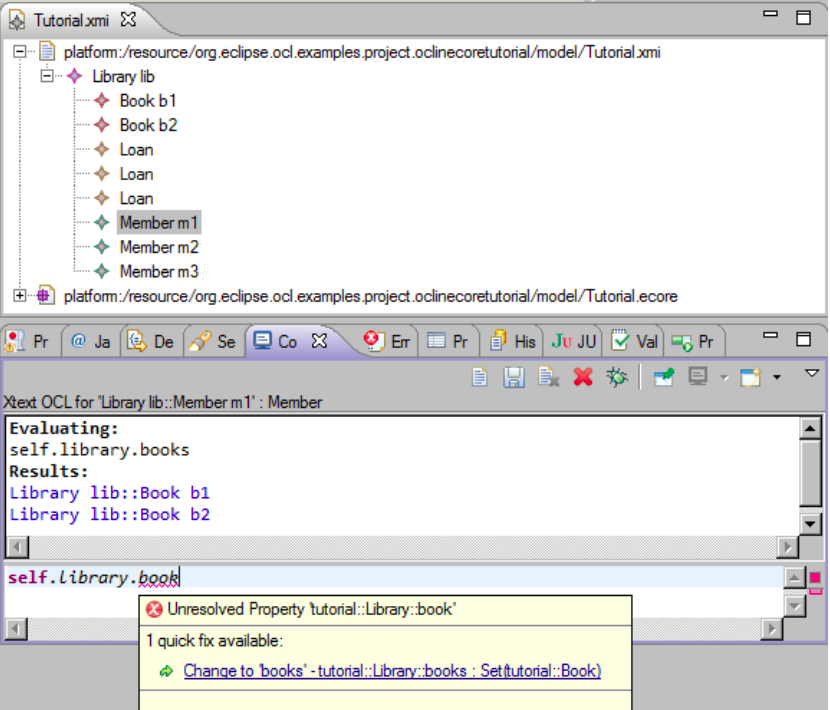
\includegraphics[width=0.7\textwidth]{Chapters/figures/4_RelatedWork/06_eclipseocl_1.png}
\caption{OCL Console~\cite{eclipseocl}}
\label{fig:07_eclipseocl_1}
\end{figure}

\begin{figure}[ht]
\centering
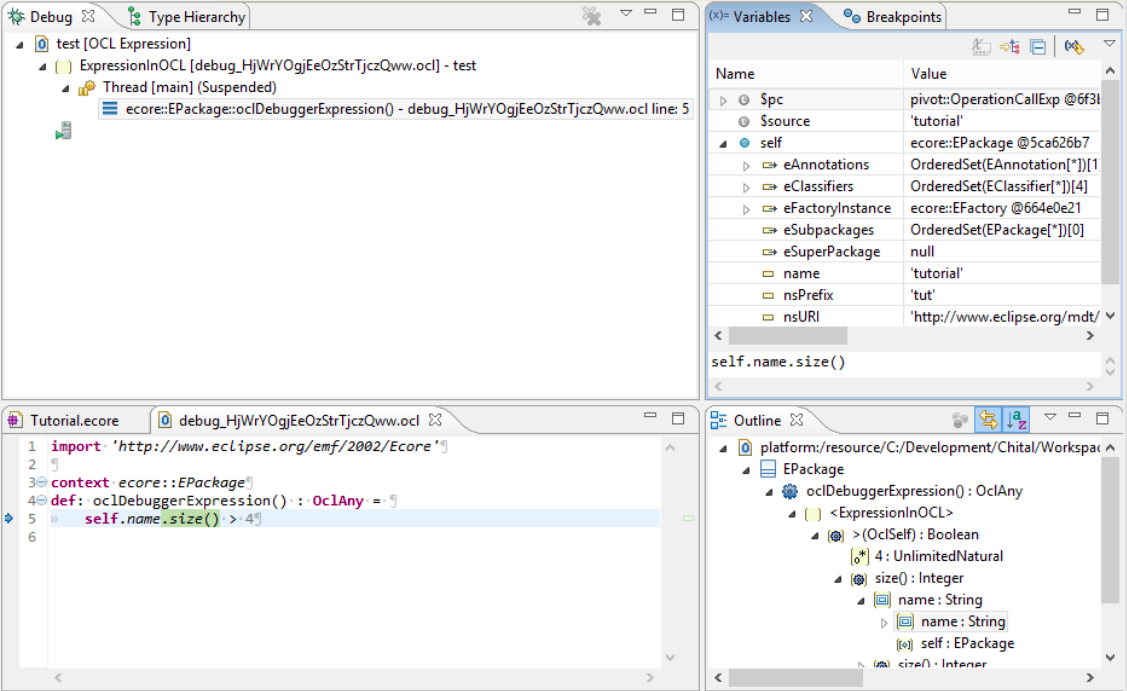
\includegraphics[width=0.7\textwidth]{Chapters/figures/4_RelatedWork/06_eclipseocl_2.png}
\caption{OCL Debugger~\cite{eclipseocl}}
\label{fig:07_eclipseocl_2}
\end{figure}

Both tools offer a wide variety of useful functionalities for modelers, but none provides syntax highlighting on elements of the UML class diagram that are referred on an OCL expression, which we believe that can soften the learning curve of this language. For our research topic, USE is the most relevant tool because it provides the basis for syntax highlighting on the UML class diagram.